\subsection{The Middleware Libraries}
\label{subsec:workloads}

%HPC libraries that sit below the applications but above the hardware fall into two primary categories: middleware libraries and communication protocol libraries. Middleware libraries sit directly above the InfiniBand network and bellow the protocol libraries to provide low-level network interfacing all the way down to the hardware. Protocol libraries implement communication standards through the use of these middlewares such as message passing or remote memory access. For this work, we will be looking at running the methodology on middleware libraries as they are the primary focus,

Three middleware libraries were selected for this work, namely Unified Communication-X (UCX), Open Fabrics Interface (OFI), and Sandia National Lab's (SNL's) implementation of Portals4 (Portals). These three were selected as they are the only known open-source HPC middlewares that have been used in production systems. Table \ref{tab:library_metadata} displays an overview of general metrics of interest related to code-base size and composition. The files counts and lines of code are divided by file type in order to give an idea as to their composition. ANTLR error counts are provided for insight into the effectiveness of the C grammar file used. A point of note is that ANTLR errors typically have a cascading effect in that one error will cause an incorrect parsing later on as the context is incorrect which causes another error. The unique file name counts are indicative of how many nodes were removed from the cluster using the same-name hierarchical methods discussed in Section \ref{subsec:graph_construction}. Declaration counts are provided to give an idea of the total number of shared dependencies within the codebase and what proportion of them is macros vs non-macros.

\begin{table*}[ht]
    \centering
    \caption{Metadata on the statistics for each of the code-bases including those related to the size of the code-base and the parsed outputs.}
    \begin{tabular}{|c|c|c|c|c|c|c|c|c|c|c|c|c|}
        \hline
            \multirow{2}{*}{Library} & \multicolumn{4}{c|}{Files} & \multicolumn{4}{c|}{Lines of Code} & ANTLR & Unique File & Macro & Non-Macro \\
        \cline{2-9}
            & All & *.c & *.h & *.inl & All & *.c & *.h & *.inl & Errors & Names & Declarations & Declarations \\
        \hline
        \hline
            UCX & 540 & 253 & 258 & 29 & 201,454 & 133,512 & 58,553 & 9,389 & 901 & 329 & 1222 & 34,176 \\
        \hline
            OFI & 1159 & 697 & 462 & 0 & 541,459 & 424,588 & 116,871 & 0 & 2088 & 1048 & 3702 & 53,708 \\
        \hline
            Portals & 217 & 135 & 82 & 0 & 60,204 & 46,149 & 14,055 & 0 & 177 & 177 & 325 & 6080 \\
        \hline
        %    SOS & 69 & 38 & 23 & 8 & 29,474 & 16,834 & 8,623 & 4017 & 1670 & 60 & 588 & 3196 \\
        %\hline
        %    OpenMPI & 1910 & 1600 & 310 & 0 & 347,772 & 283,853 & 63,919 & 0 & 3567 & 1777 & 965 & 40,548 \\
        %\hline
        \hline
            UCT & 205 & 103 & 98 & 4 & 84,339 & 57,732 & 23,722 & 2,885 & -  & - & 297 & 14,976 \\
        \hline
            UCP & 137 & 71 & 46 & 20 & 67,674 & 47,474 & 14,390 & 5,820 & -  & - & 161 & 13,077 \\
        \hline
            UCS & 198 & 79 & 114 & 5 & 49441 & 283,306 & 20,451 & 684 & -  & - & 764 & 6,123 \\
        \hline
    \end{tabular}
    \label{tab:library_metadata}
\end{table*}


What follows is a description of the three middleware libraries of interest in order to give context for the analyses in Section \ref{subsec:arch_extraction}. Extra analysis is provided for UCX in Section \ref{subsec:ucx_arch} so the description for it is a bit more in-depth as to it's component's inner workings than the other two. Table \ref{tab:library_metadata} also includes a breakdown of the UCX data for each of its individual components.

UCX \cite{ucx_github} is an open-source communication framework developed by NVIDIA with wide-spread adoption in HPC systems and having other proprietary HPC network fabrics being built on top of it \cite{openfabrics_libfabric}. UCX is the most notorious for its code complexity and lack of documentation out of the code-bases selected which is why it was selected for a deeper analysis. UCX has three primary components which are highly interconnected with one another:
\begin{itemize}
    \item Protocols (UCP) - implements high-level protocols (e.g. MPI) to expose the capabilities of UCT to the application
    \item Transport (UCT) - abstracts the hardware architecture to enable communication protocols over the network
    \item Service (UCS) - provides the functionality for implementing portable and efficient utilities with OS bypassing for direct memory management
\end{itemize}

Portals \ref{portals4_repo} is a modular network middleware implementation of the Portals 4 standard \ref{portals4.3} that focuses on providing communication libraries with the tools they need to implement any protocol. The Portals 4 standard was developed by SNL as an alternative to UCX which sought to provide communication libraries with a more sophisticated suite of tool. Portals is a lightweight option that was deployed on systems at US national labs as a proof of concept as to the possibilities of the Portals 4 standard as a middleware. OFI \cite{libfabric_repo} is an implementation of the Portals 4 standard that was deployed by Intel in a collaboration with SNL following Portals' success. It is actively maintained by Intel and used on production systems. Portals in no longer actively maintained as a result of OFI's success.

%\begin{figure*}[ht]
%    \centering
%    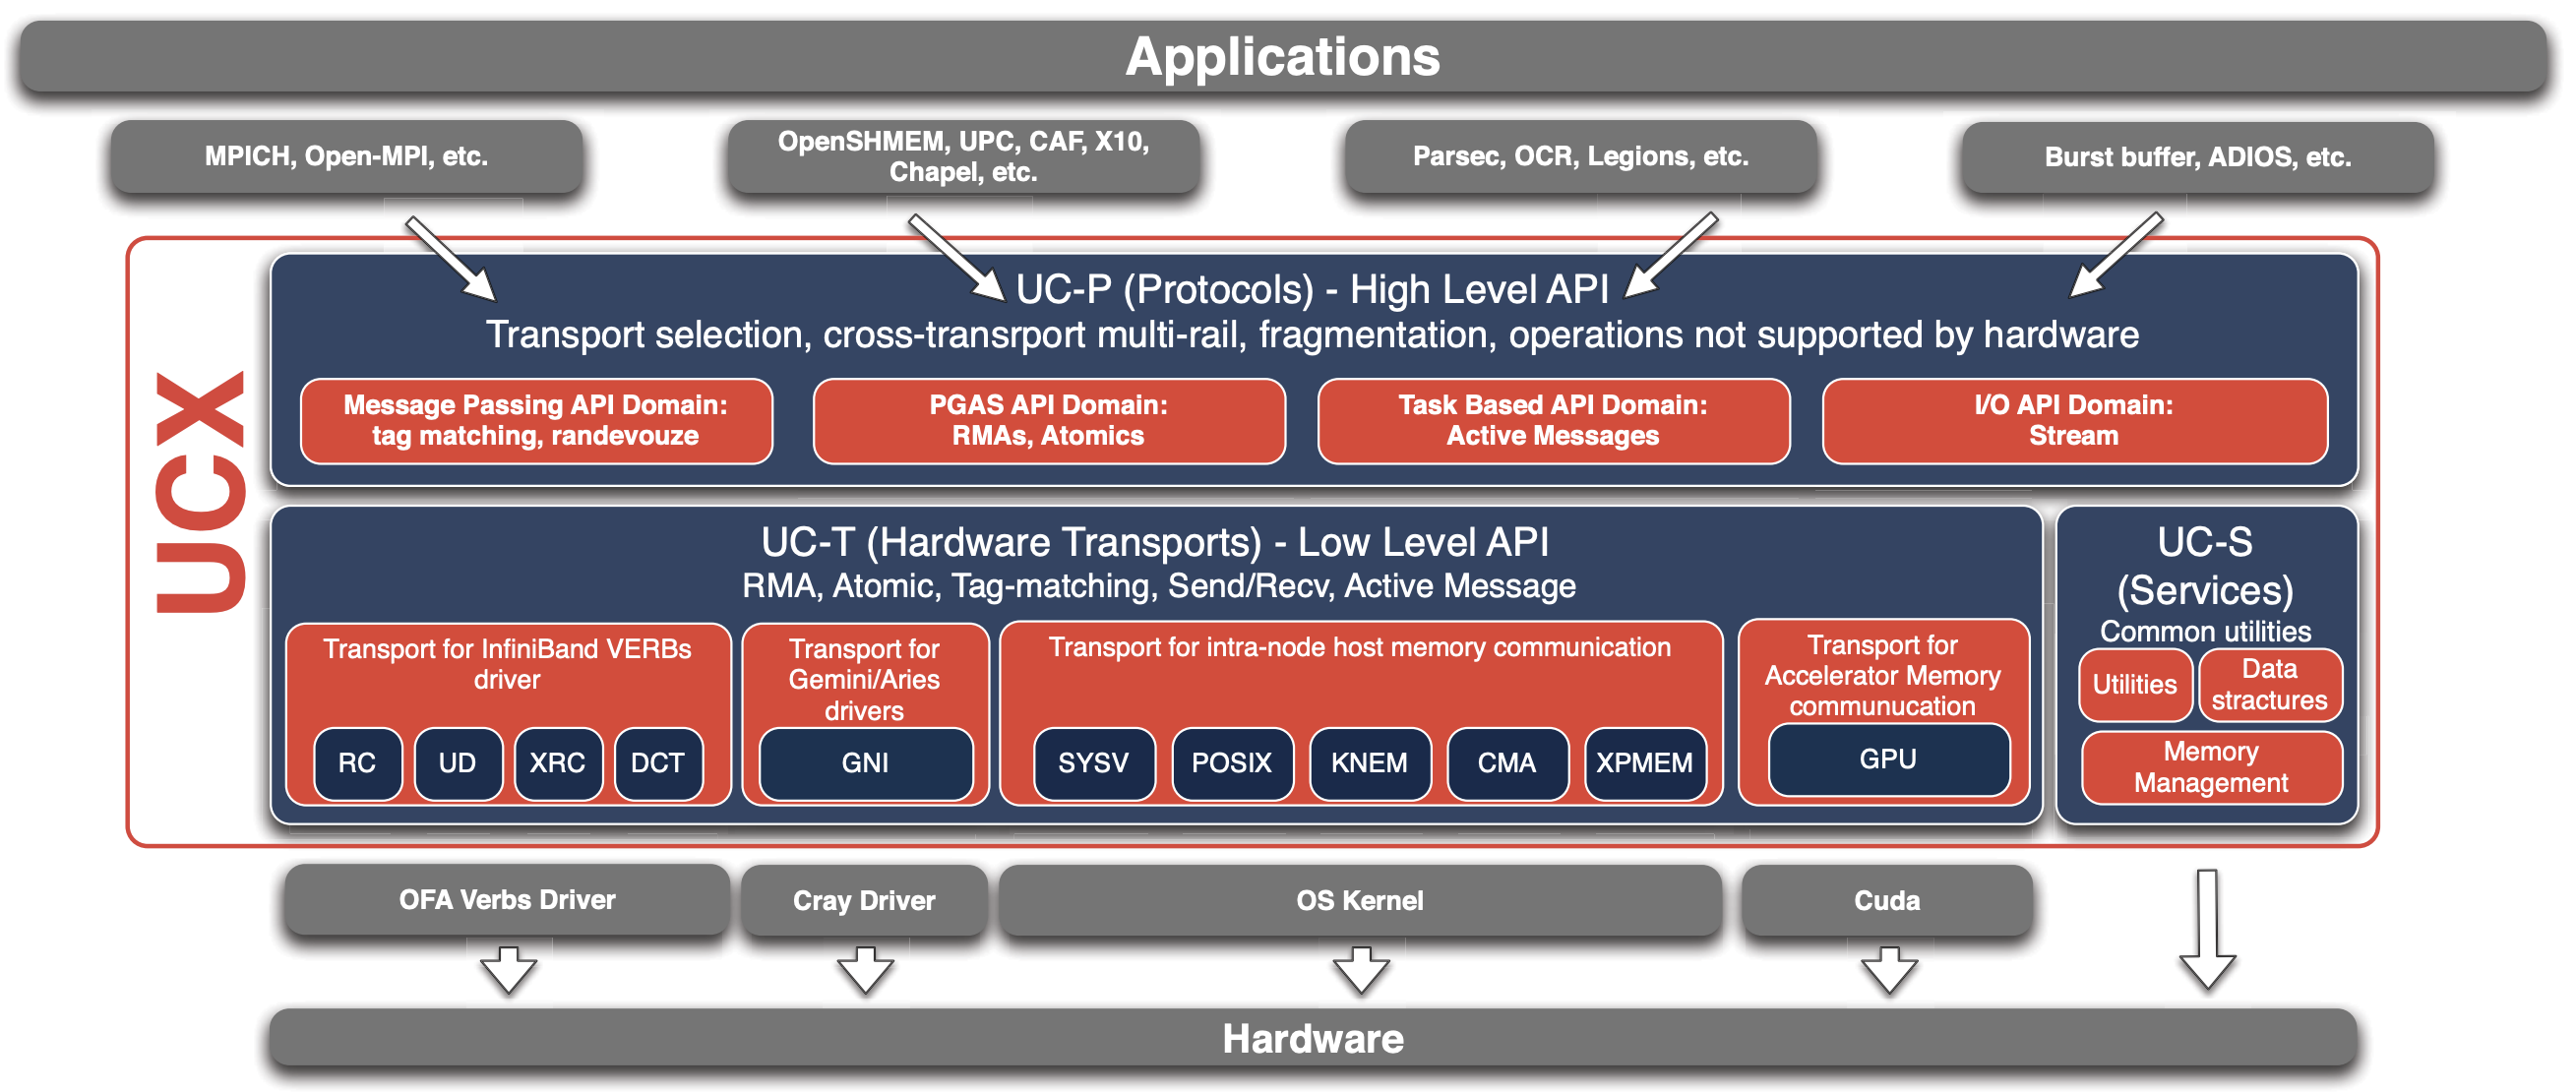
\includegraphics[width=1.0\linewidth]{figures/ucx_structure.png} \\
%    \caption{A high-level overview of the UCX architecture taken from the original paper \cite{ucx_paper}.}
%    \label{fig:ucx_struct}
%\end{figure*}
